
\section{Ronda 3: el atlas completo de mixers}
\label{sec:annex-experiment-3}

Este apéndice reporta la ronda~3 en su totalidad. La ronda~2 midió 868 configuraciones y dejó vacías 194 de las 861 celdas híbridas; la ronda~3 cierra la matriz. La campaña entrenó todos los pares no ordenados de los $54$ mixers registrados---$\binom{54}{2}=1{,}431$ celdas, sin ninguna ausente---más $54$ líneas base de un solo mixer y $168$ corridas de ablación que mueven un interruptor a la vez (familia de optimizador, normalización, codificación posicional, enrutamiento MoE, camino residual, tarea y clase de modelo). Es la medición más grande del proyecto: $1{,}653$ corridas de entrenamiento, $20,5$ millones de pasos de optimización registrados y $3{,}668$ horas de tiempo de pared de entrenamiento repartidas en $7,2$ días calendario.

El apéndice sigue el orden del análisis: la población y sus advertencias, el paisaje de parámetros, los resultados de entrenamiento, la dinámica de aprendizaje, la presión del gradiente por bloque, el coste del entrenamiento, las mediciones de inferencia y cuantización, la fiabilidad del pipeline y las correlaciones entre las variables medidas. Todos los números los regenera \texttt{make\_report.py} a partir de \texttt{master.csv}; todas las figuras las regenera \texttt{make\_paper\_figures.py} con los mismos constructores que el resto del informe, así que este texto y los artefactos no pueden contradecirse.

\subsection{Configuración, población y exclusiones}

El harness produjo $12{,}820$ registros de etapa: $1{,}653$ intentos de entrenamiento, $4{,}686$ exportaciones a Transformers, $5{,}146$ evaluaciones de inferencia, $1{,}334$ registros de despliegue y una conversión BitNet/GGUF. El entrenamiento tuvo éxito $1{,}643$ veces y falló $10$ veces; los fallos son diez pares con \texttt{engram} que terminan con un código distinto de cero y se discuten en la Sección~\ref{sec:r3-reliability}. La población se resume en la Tabla~\ref{tab:r3-families}.

\begin{table}[H]
\centering
\small
\caption{Población de la ronda~3 por familia: corridas, corridas excluidas como pruebas de humo (menos de 100 épocas), mediana de épocas y parámetros de las corridas analizadas, mediana de la pérdida final, minutos por Mparámetro y tasa de éxito del entrenamiento.}
\label{tab:r3-families}
\begin{tabular}{lrrrrrrr}
\toprule
Familia & $n$ & Humo & Épocas & Parám. (M) & Pérdida & min/Mparám & OK \\
\midrule
pares híbridos & 1{,}431 & 22 & 459 & 0,32 & 8,778 & 421,5 & 99,3\% \\
mixers únicos & 54 & 0 & 382 & 0,26 & 8,998 & 546,5 & 100,0\% \\
optimizadores & 39 & 0 & 312 & 0,31 & 9,321 & 311,5 & 100,0\% \\
ablaciones de PE de texto & 12 & 1 & 370 & 0,31 & 8,826 & 297,2 & 100,0\% \\
ablaciones de PE del ViT & 39 & 0 & 499 & 0,35 & 1,004 & 207,8 & 100,0\% \\
tareas de visión & 9 & 0 & 499 & 0,34 & 1,004 & 244,3 & 100,0\% \\
tareas de audio & 4 & 1 & 499 & 0,45 & 1,098 & 23,6 & 100,0\% \\
ejecuciones con datos reales & 8 & 0 & 499 & 0,33 & 1,099 & 84,9 & 100,0\% \\
tokenizadores & 4 & 0 & 499 & 0,31 & 6,130 & 31,5 & 100,0\% \\
interruptores de arquitectura & 23 & 4 & 370 & 0,31 & 8,942 & 318,1 & 100,0\% \\
variantes MoE & 17 & 15 & 499 & 0,37 & 8,873 & 556,3 & 100,0\% \\
normalización & 6 & 0 & 312 & 0,31 & 8,944 & 237,0 & 100,0\% \\
tamaño de lote & 2 & 0 & 406 & 0,31 & 8,669 & 238,1 & 100,0\% \\
interruptores de tarea & 4 & 0 & 499 & 0,31 & 6,426 & 265,0 & 100,0\% \\
\bottomrule
\end{tabular}
\end{table}

Dos exclusiones condicionan el resto del apéndice. Primero, la etapa de \emph{despliegue} no se analiza. En esta ronda el desplegador recibió la dataclass viva \texttt{FrankensteinModelConfig} guardada en el checkpoint donde esperaba un diccionario y le llamó \texttt{.get()}, así que $822$ de los $1{,}334$ registros de despliegue fallaron con \texttt{'FrankensteinModelConfig' object has no attribute 'get'}. Medir una etapa rota confundiría un error de serialización con la calidad de la cuantización; por eso el despliegue se descarta y el análisis de pesos cuantizados usa la ruta de exportación a Transformers, que exportó $4{,}686$ modelos sin fallos. Segundo, solo $662$ de las corridas produjeron filas de inferencia de Hugging Face ($33{,}380$ filas de muestra sobre $653$ pares MLM más unas pocas corridas de LM causal y clasificación de texto); la sección de inferencia estudia ese subconjunto, no el atlas completo.

Las corridas son heterogéneas de una forma que importa para las curvas. Las configuraciones piden 500 épocas, pero el harness detiene una corrida antes (por calendario, criterio de meseta o un tope específico de la ablación): $734$ corridas llegaron a la última época y $919$ se detuvieron antes. Por eso las curvas de aprendizaje se estiran sobre el progreso propio de cada corrida en lugar de dibujarse contra pasos absolutos, de modo que una corrida de 300 épocas y una de 500 se comparan en la misma fracción de su calendario. El análisis de rendimiento y coste conserva los tiempos absolutos, porque eso es lo que pagó la campaña. Las 61 corridas con menos de 5{,}000 pasos registrados están dominadas por las familias de audio, tokenizadores y datos reales, cuyos conjuntos son lo bastante pequeños como para terminar en segundos. Una distinción más fuerte importa para todas las comparaciones que siguen: $44$ corridas se detuvieron antes de la época~100---quince de las diecisiete ablaciones MoE (pruebas de humo de enrutamiento de cinco épocas), la única conversión BitNet/GGUF, veintidós pares truncados y un puñado de ablaciones de interruptores y de PE. Permanecen en la población y en el registro de cómputo, pero todos los resultados de pérdida, dinámica, gradiente, coste por corrida y correlación se calculan sobre las $1{,}609$ corridas con al menos 100 épocas. La columna de presupuesto de la Tabla~\ref{tab:r3-families} hace visible la distinción.

\begin{figure}[tbp]
\centering
\fitfigure{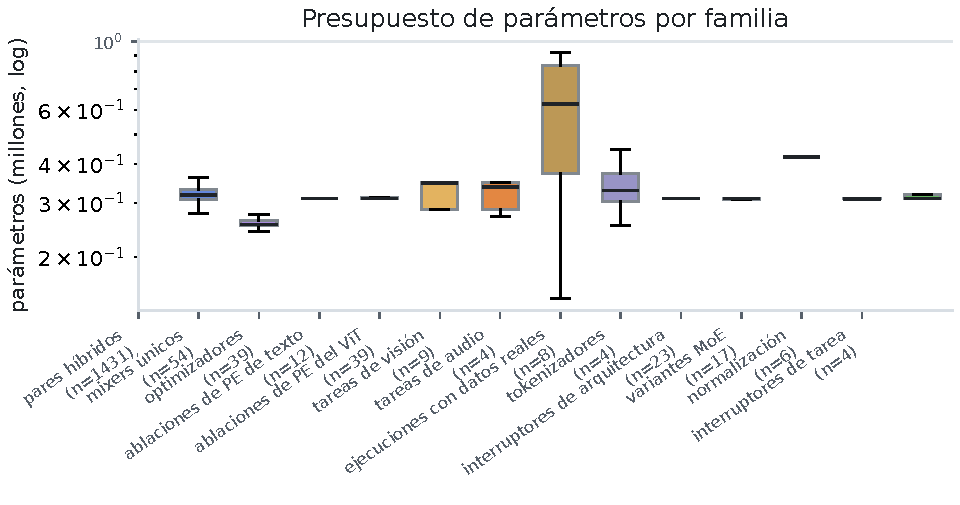
\includegraphics{../paper/figures/experiments/round3/params_family_box-es.pdf}}
\caption{Presupuesto de parámetros por familia (escala logarítmica).}
\label{fig:r3-params-family}
\end{figure}
\begin{figure}[tbp]
\centering
\fitfigure{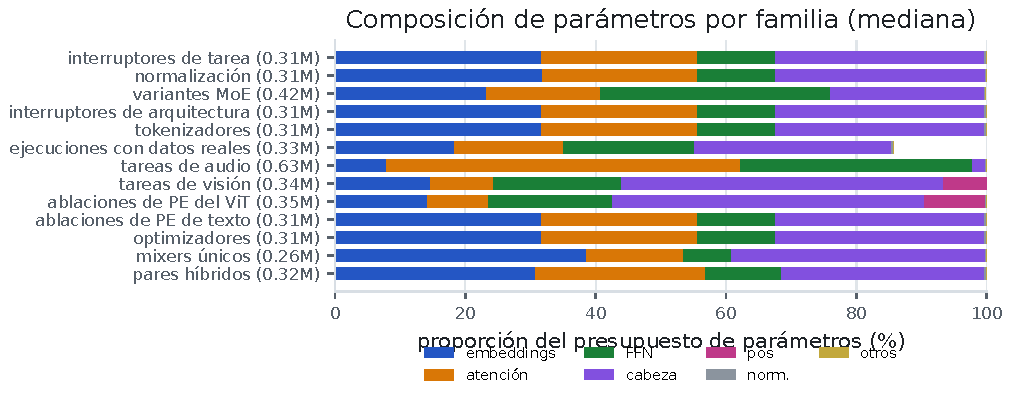
\includegraphics{../paper/figures/experiments/round3/params_composition-es.pdf}}
\caption{Dónde viven los parámetros, por familia. Los embeddings y la cabeza son costes fijos; la atención y la FFN concentran las diferencias arquitectónicas.}
\label{fig:r3-params-composition}
\end{figure}

\subsection{El paisaje de parámetros}

Las $1{,}653$ corridas abarcan de $147{,}171$ a $1{,}957{,}440$ parámetros (mediana $315{,}744$). La corrida mediana se sitúa en $315{,}744$ parámetros y el par híbrido mediano en $318{,}784$, con una composición casi independiente de la familia: el embedding de tokens y la cabeza de salida son costes fijos de aproximadamente $31,0\%$ y $31,6\%$ del presupuesto, la atención toma $24,8\%$, la FFN $11,8\%$ y las capas de normalización $0,3\%$. La decisión arquitectónica mueve, por tanto, un cuarto de los parámetros; los otros tres cuartos son el precio de tener vocabulario y clasificador. Los transformers de visión son la excepción: los embeddings de parches reemplazan al embedding de tokens y la cabeza de clasificación es pequeña, así que su presupuesto lo dominan la atención y la FFN.

El coste por mixer tiene una lectura clara, y no es la que se adivinaría desde la literatura. Los segundos mixers más baratos son \texttt{mamba} (0,28M), \texttt{ccgqa} (0,29M), \texttt{cca} (0,29M); los más caros son \texttt{gmla} (1,67M), \texttt{engram} (0,60M), \texttt{mfa} (0,54M). \texttt{engram} paga su banco de memoria clave--valor y \texttt{gmla} paga las proyecciones latentes de la atención latente multimando con compuerta. Barato no predice bueno: \texttt{ccgqa} y \texttt{gqa} están entre los más baratos y terminan algo por debajo de la mediana de los pares, mientras \texttt{mamba}, \texttt{cca} y \texttt{mlra} son igual de baratos y terminan por encima; \texttt{engram} paga 0,28M parámetros extra por una pérdida indistinguible de la mediana.

La dispersión de la pérdida final contra el número de parámetros (Figura~\ref{fig:r3-params-loss}) tiene una correlación de rango de $-0,42$ sobre los $1{,}431$ pares: los modelos más grandes son algo mejores, pero el tamaño explica solo una sexta parte del orden, y el atlas abarca más de un factor diez de tamaño frente a dos nats de pérdida. El presupuesto ayuda; no decide. Es la misma conclusión de la ronda~2, ahora medida sobre la rejilla completa en lugar de sobre dos tercios de ella.

\begin{figure}[tbp]
\centering
\fitfigure{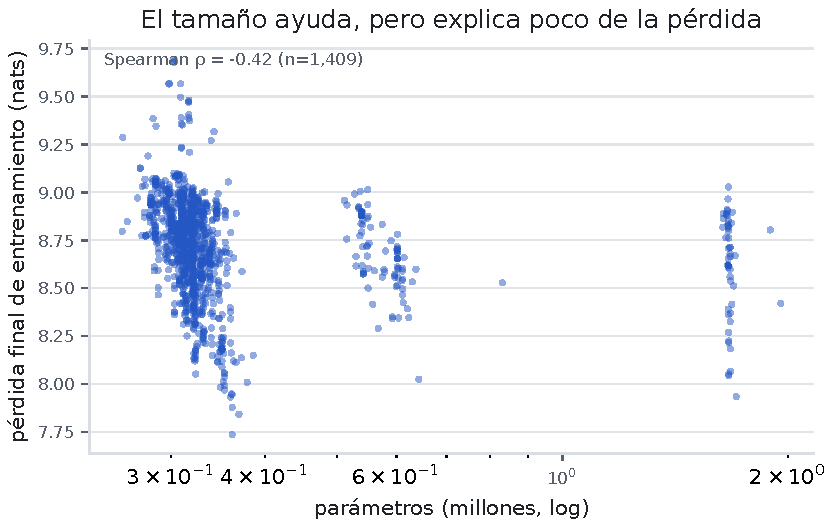
\includegraphics{../paper/figures/experiments/round3/params_vs_loss-es.pdf}}
\caption{Pérdida final de entrenamiento contra número de parámetros para los pares híbridos.}
\label{fig:r3-params-loss}
\end{figure}

\subsection{Resultados de entrenamiento}

Los pares híbridos terminan con una pérdida final mediana de $8,78$ nats (de $7,74$ a $9,70$), el mejor es $\texttt{attn\_falcon2a\_\_conformer}$ con $7,736$ y el peor $\texttt{attn\_mtla\_\_tpa}$ con $9,70$. La Tabla~\ref{tab:r3-top-loss} lista los diez mejores pares. La dispersión es amplia: la diferencia entre el mejor y el peor par es mayor que la diferencia entre la mejor ablación de optimizador, normalización o codificación posicional y la mediana de su familia. La pila de mixers es la decisión de diseño dominante de la ronda, exactamente como en la ronda~2.

\begin{table}[H]
\centering
\small
\caption{Las diez mejores parejas híbridas por pérdida final de entrenamiento.}
\label{tab:r3-top-loss}
\begin{tabular}{rlrrr}
\toprule
\# & Pareja & Parám. (M) & Pérdida & Horas \\
\midrule
1 & \texttt{attn\_falcon2a\_\_conformer} & 0,36 & 7,736 & 2,75 \\
2 & \texttt{attn\_hgrn2\_\_conformer} & 0,37 & 7,842 & 1,87 \\
3 & \texttt{attn\_falcon2\_\_conformer} & 0,36 & 7,878 & 2,88 \\
4 & \texttt{attn\_nsa\_\_conformer} & 0,36 & 7,931 & 2,72 \\
5 & \texttt{attn\_conformer\_\_gmla} & 1,71 & 7,934 & 3,51 \\
6 & \texttt{attn\_gated\_deltanet\_\_conformer} & 0,36 & 7,945 & 2,88 \\
7 & \texttt{attn\_kda\_\_conformer} & 0,36 & 7,948 & 2,30 \\
8 & \texttt{attn\_falcon1a\_\_conformer} & 0,35 & 7,969 & 2,73 \\
9 & \texttt{attn\_gated\_deltanet2\_\_falcon2a} & 0,35 & 7,984 & 2,36 \\
10 & \texttt{attn\_falcon3a\_\_conformer} & 0,35 & 7,991 & 2,83 \\
\bottomrule
\end{tabular}
\end{table}
\begin{figure}[tbp]
\centering
\fitfigure{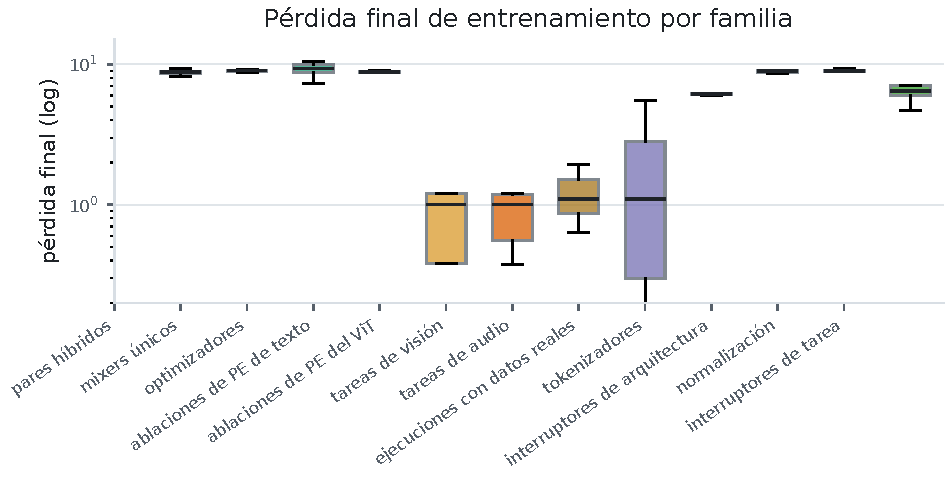
\includegraphics{../paper/figures/experiments/round3/loss_family_box-es.pdf}}
\caption{Pérdida final de entrenamiento por familia. Las tareas no son comparables entre familias; el eje logarítmico las mantiene visibles.}
\label{fig:r3-loss-family}
\end{figure}

La pérdida no es comparable entre familias porque cambia la tarea: las familias MLM se sitúan en 8,8--9,3 nats, las de visión en torno a 1,0, las de audio y datos reales en torno a 1,0 (entropía cruzada sobre otro espacio de etiquetas) y los tokenizadores en 6,0. La Figura~\ref{fig:r3-loss-family} las mantiene en eje logarítmico por esa razón. Las ablaciones MoE necesitan la advertencia de presupuesto: las quince variantes de enrutamiento de cinco épocas nunca salen de la primera época y quedan excluidas, así que solo las dos variantes de calendario completo---\texttt{moe\_interleaved} y \texttt{moe\_latent}---son comparables con la población de pares, donde aterrizan en la mediana. El estudio de enrutamiento es, por tanto, una prueba de humo en esta ronda y no evidencia sobre la capacidad de los expertos.

La calidad retenida se mide con las filas de inferencia. Sobre los $653$ pares MLM, la exactitud top-1 media es $4,46\%$ y el acierto top-5 medio es $24,0\%$; las medianas son 0 y 28,6\%, así que la distribución mezcla unos pocos pares que aprendieron algo con una mayoría que no. La Tabla~\ref{tab:r3-top-inference} lista los mejores pares. La correlación de rango entre la pérdida final de entrenamiento y el top-5 retenido es solo $+0,14$: una pérdida menor no implica un modelo mejor a esta escala, la misma advertencia de la ronda~2, ahora sobre 653 pares en lugar de 667.

\begin{table}[H]
\centering
\small
\caption{Los diez mejores pares por acierto top-5 retenido (exportación sin cuantizar).}
\label{tab:r3-top-inference}
\begin{tabular}{rlrrr}
\toprule
\# & Pareja & Top-1 & Top-5 & Pérdida final \\
\midrule
1 & \texttt{attn\_bigbird\_\_ccgqa} & 0,00\% & 42,9\% & 8,784 \\
2 & \texttt{attn\_bigbird\_\_sparsek} & 0,00\% & 42,9\% & 8,649 \\
3 & \texttt{attn\_bigbird\_\_ssog} & 0,00\% & 42,9\% & 8,732 \\
4 & \texttt{attn\_cca\_\_gmla} & 0,00\% & 42,9\% & 8,889 \\
5 & \texttt{attn\_cca\_\_kda} & 0,00\% & 42,9\% & 8,718 \\
6 & \texttt{attn\_ccgqa\_\_ca} & 14,29\% & 42,9\% & 8,764 \\
7 & \texttt{attn\_ccgqa\_\_falcon2} & 14,29\% & 42,9\% & 8,656 \\
8 & \texttt{attn\_ccgqa\_\_falcon2a} & 14,29\% & 42,9\% & 8,551 \\
9 & \texttt{attn\_ccgqa\_\_fastconformer} & 14,29\% & 42,9\% & 8,761 \\
10 & \texttt{attn\_ccgqa\_\_kpa} & 14,29\% & 42,9\% & 8,963 \\
\bottomrule
\end{tabular}
\end{table}

\subsection{Dinámica de aprendizaje}

La Figura~\ref{fig:r3-curves-quantiles} muestra la curva de la población. El par mediano empieza en $10,50$ nats y termina en $8,78$; la banda P10--P90 al final es $8,41$--$8,97$, más estrecha que la dispersión entre familias. La mayor parte de la reducción ocurre en el primer cuarto: la mediana alcanza $9,47$ al 25\% del calendario, $8,92$ a la mitad y $8,75$ a las tres cuartas partes. La ronda~3 mide, por tanto, cuán rápido aprende una configuración, no dónde converge: las curvas siguen bajando cuando termina el calendario.

\begin{figure}[tbp]
\centering
\fitfigure{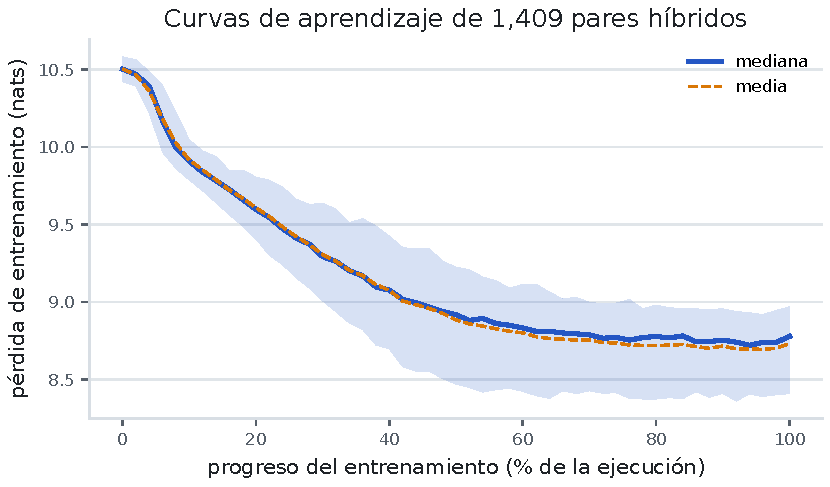
\includegraphics{../paper/figures/experiments/round3/curves_quantiles-es.pdf}}
\caption{Curvas de aprendizaje de la población con banda P10--P90, normalizadas al calendario propio de cada corrida.}
\label{fig:r3-curves-quantiles}
\end{figure}
\begin{figure}[tbp]
\centering
\fitfigure{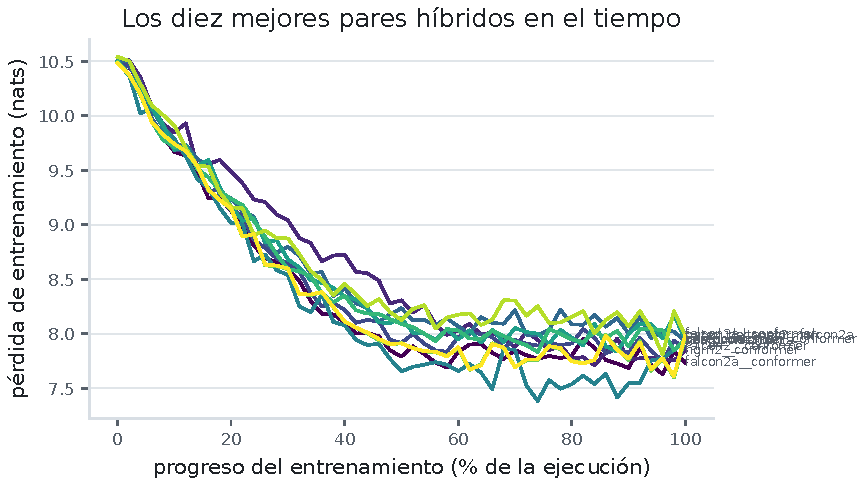
\includegraphics{../paper/figures/experiments/round3/curves_top10-es.pdf}}
\caption{Los diez mejores pares híbridos sobre su propio calendario de entrenamiento.}
\label{fig:r3-curves-top10}
\end{figure}

El orden de los mejores pares se establece temprano. Al cuarto del calendario la pérdida por par ya ordena los pares con una correlación de Spearman de $0,62$ frente a su orden final, y en la Figura~\ref{fig:r3-curves-top10} los diez mejores se separan de la población antes de la mitad y rara vez se cruzan después. El número de épocas necesarias para alcanzar el 90\% de la caída total de pérdida de una corrida lo confirma: la mediana es $41\%$ del calendario, y las medianas por familia van desde $21\%$ en las tareas de visión (donde la pérdida colapsa casi de inmediato) hasta $56\%$ en las ablaciones de normalización (donde las diferencias entre normas solo aparecen tarde). Los pares híbridos se sitúan en $40\%$.

\begin{figure}[tbp]
\centering
\fitfigure{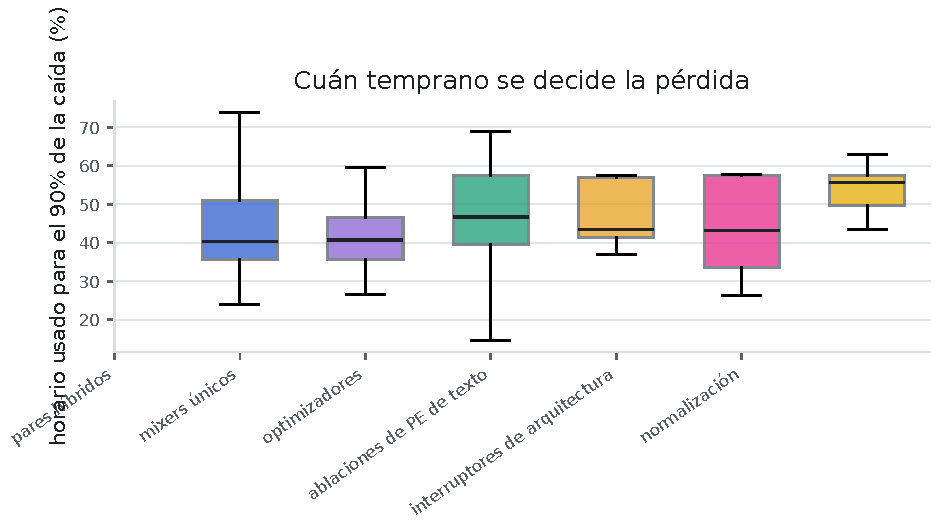
\includegraphics{../paper/figures/experiments/round3/convergence_speed-es.pdf}}
\caption{Fracción del calendario necesaria para alcanzar el 90\% de la caída total de pérdida, por familia.}
\label{fig:r3-convergence}
\end{figure}

\subsection{Presión del gradiente por bloque de parámetros}

El entrenador registra la norma L2 del gradiente de cada bloque de parámetros después del recorte: embeddings, codificación posicional, atención, FFN, normalización, cabeza, mHC, router, residual y otros. La Tabla~\ref{tab:r3-gradients} reproduce las medianas y la Figura~\ref{fig:r3-grad-groups} las trayectorias durante el entrenamiento.

\begin{table}[H]
\centering
\small
\caption{Norma del gradiente por bloque de parámetros: mediana de la media por corrida, mediana del último paso, coeficiente de variación y fracción de corridas con bloque activo.}
\label{tab:r3-gradients}
\begin{tabular}{lrrrr}
\toprule
Bloque & Media & Final & CV & Activo \\
\midrule
embeddings & 0,152 & 0,163 & 0,27 & 99,9\% \\
posicional & 0,000 & 0,000 & 1,79 & 3,5\% \\
atención & 2,121 & 2,503 & 0,22 & 100,0\% \\
FFN & 0,709 & 0,674 & 0,31 & 100,0\% \\
normalización & 0,326 & 0,336 & 0,13 & 99,9\% \\
cabeza & 3,657 & 3,733 & 0,13 & 100,0\% \\
mHC & 0,000 & 0,000 & 0,03 & 0,1\% \\
router & 0,000 & 0,000 & 0,50 & 1,2\% \\
residual & 0,000 & 0,000 & 0,82 & 0,1\% \\
otros & 0,000 & 0,000 & n/a & 0,0\% \\
\bottomrule
\end{tabular}
\end{table}
\begin{figure}[tbp]
\centering
\fitfigure{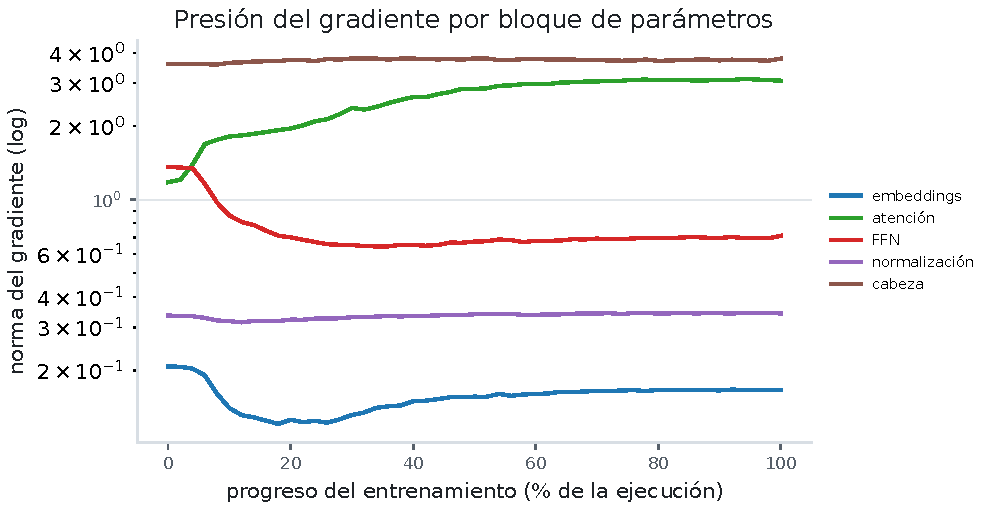
\includegraphics{../paper/figures/experiments/round3/grad_groups_curves-es.pdf}}
\caption{Norma del gradiente mediana por bloque de parámetros durante el entrenamiento (post-recorte).}
\label{fig:r3-grad-groups}
\end{figure}

Tres hechos destacan. Primero, la cabeza soporta el gradiente mayor ($3,66$ de media, $3,73$ al final), seguida de la atención ($2,12$, $2,50$) y la FFN ($0,71$, $0,67$); los embeddings y la normalización son un orden de magnitud menores ($0,15$ y $0,33$). El orden es estable en toda la campaña, y por eso la normalización por bloque del optimizador no es una elección cosmética. Segundo, los coeficientes de variación son pequeños---$0,13$ para la cabeza, $0,22$ para la atención, $0,31$ para la FFN---así que la escala del gradiente de un bloque es una propiedad de la arquitectura, no del paso. Tercero, los bloques que solo existen en algunas configuraciones (\texttt{mhc}, \texttt{router}, \texttt{residual}) valen exactamente cero en las corridas que no los activan, lo que hace que las filas de mediana cero de la tabla sean informativas y no datos faltantes.

\begin{figure}[tbp]
\centering
\fitfigure{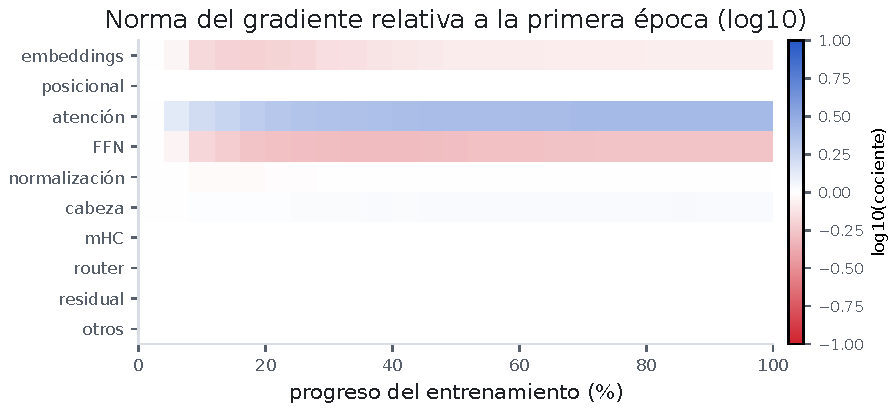
\includegraphics{../paper/figures/experiments/round3/grad_heatmap-es.pdf}}
\caption{Norma del gradiente por bloque relativa a su primera época, en unidades log10.}
\label{fig:r3-grad-heatmap}
\end{figure}

El mapa de calor (Figura~\ref{fig:r3-grad-heatmap}) lee las mismas estadísticas en función del progreso. La cabeza es plana, la atención crece ligeramente y la FFN decae por un factor de aproximadamente dos durante la primera mitad del entrenamiento antes de estabilizarse; los embeddings decaen a medida que se aprenden las estadísticas del vocabulario. Nada explota: no hay pasos con NaN en toda la campaña, hay $109$ pasos con Inf (todos reparados en el sitio, en $15$ corridas) y el coeficiente de variación de la norma del gradiente se relaciona inversamente con la pérdida final ($-0,61$), es decir, las corridas que terminan más abajo tienen gradientes algo más variables, no menos.

\begin{figure}[tbp]
\centering
\fitfigure{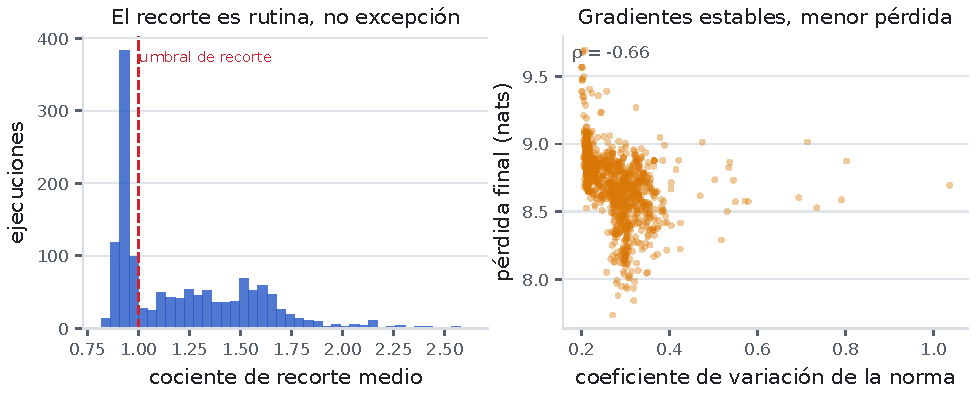
\includegraphics{../paper/figures/experiments/round3/grad_health-es.pdf}}
\caption{Distribución del cociente de recorte y variabilidad del gradiente contra la pérdida final.}
\label{fig:r3-grad-health}
\end{figure}

El recorte, sin embargo, es rutina y no excepción. La mediana del cociente de recorte medio es $1,04$---justo por encima del umbral 1---y $51,6\%$ de las corridas pasan la campaña recortando de media, con un P90 de $1,65$. La ronda~2 reportó una mediana de 0,90 y un recorte excepcional; la diferencia es el calendario más largo y las tasas de aprendizaje más altas de la ronda~3. La consecuencia para el informe es que las normas de gradiente deben leerse como normas después del recorte, que es lo que registra el entrenador.

El consumo de memoria es modesto: la corrida mediana alcanza un pico de $1{,}457$ MB de memoria residente y el máximo es $3{,}159$ MB, así que el atlas completo cabe en un solo host de CPU con una docena de workers.

\subsection{Rendimiento y coste}

El tiempo de entrenamiento crece solo débilmente con los parámetros: un ajuste log-log sobre los pares MLM da un exponente de $0,25$ con $R^2=0,06$. La razón es que lo que mide el reloj no es el número de parámetros---dominan el número de pasos, y el número de pasos varía por familia y por parada temprana. El coste normalizado (Figura~\ref{fig:r3-cost-mparam}) es la cantidad que compara arquitecturas con justicia: la corrida mediana gasta $402$ minutos por millón de parámetros, y las medianas por familia se mueven en un factor de aproximadamente tres alrededor de ese valor. Un par híbrido cuesta $422$ minutos por Mparámetro, algo por debajo de una línea base de un solo mixer ($547$) y por encima de una ablación de optimizador ($311$); las diferencias vienen del calendario efectivo y del coste de la actualización, no del número de parámetros.

\begin{figure}[tbp]
\centering
\fitfigure{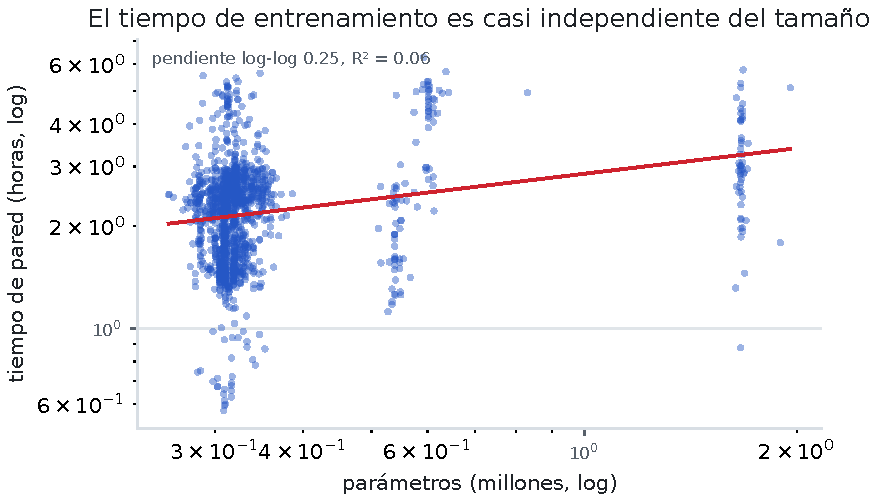
\includegraphics{../paper/figures/experiments/round3/time_vs_params-es.pdf}}
\caption{Tiempo de pared de entrenamiento contra número de parámetros, con el ajuste log-log.}
\label{fig:r3-time-params}
\end{figure}
\begin{figure}[tbp]
\centering
\fitfigure{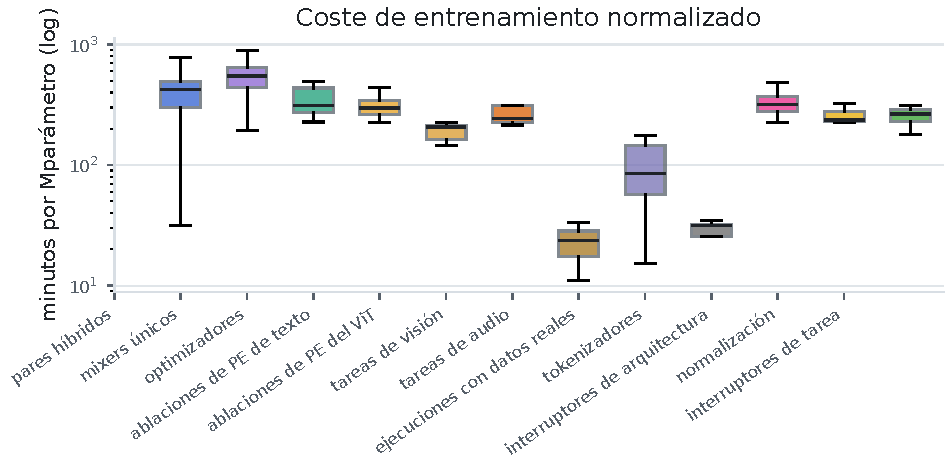
\includegraphics{../paper/figures/experiments/round3/cost_per_mparam-es.pdf}}
\caption{Minutos de entrenamiento por millón de parámetros, por familia.}
\label{fig:r3-cost-mparam}
\end{figure}
\begin{figure}[tbp]
\centering
\fitfigure{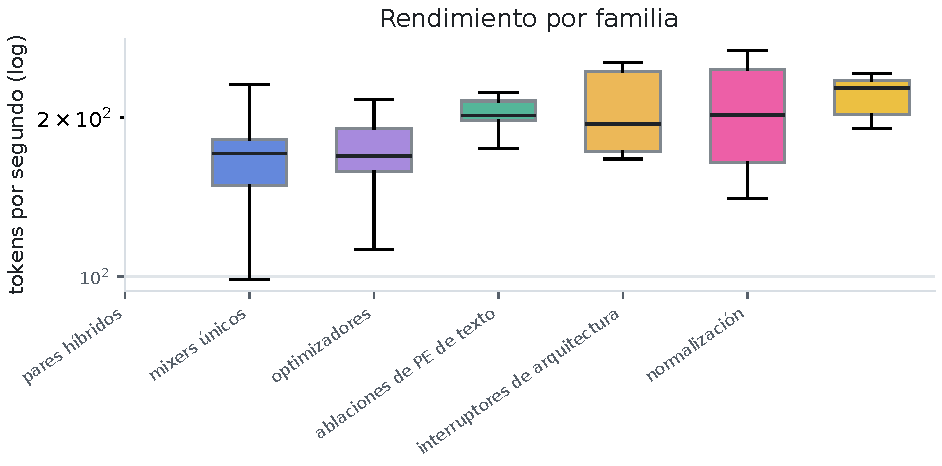
\includegraphics{../paper/figures/experiments/round3/throughput_family-es.pdf}}
\caption{Rendimiento de registro por familia (tokens por segundo, escala logarítmica).}
\label{fig:r3-throughput}
\end{figure}
\begin{figure}[tbp]
\centering
\fitfigure{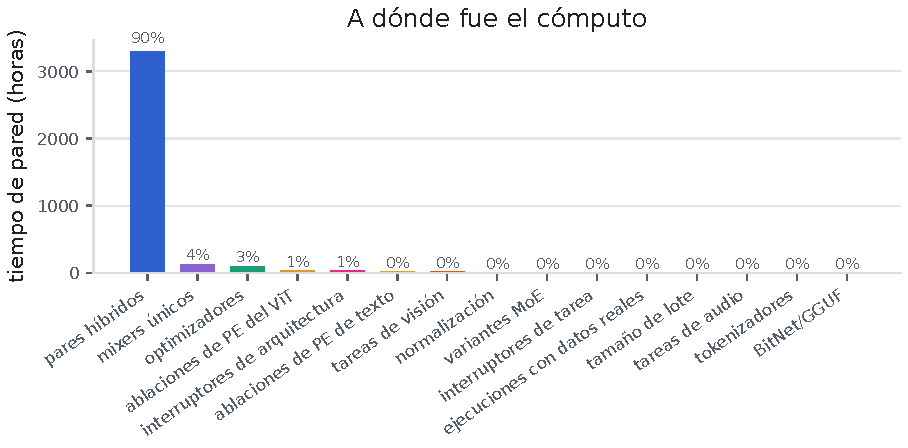
\includegraphics{../paper/figures/experiments/round3/compute_by_family-es.pdf}}
\caption{Proporción del tiempo de pared de entrenamiento por familia.}
\label{fig:r3-compute}
\end{figure}

La Figura~\ref{fig:r3-compute} muestra a dónde fueron las $3{,}668$ horas. Los pares híbridos consumen el $90,0\%$ de la campaña ($3{,}301$ horas), las líneas base de un solo mixer el $3,6\%$ y todas las demás familias menos del 3\%. Las familias de visión y audio son baratas en tiempo de pared pese a sus calendarios largos porque sus pasos son cortos; el panel de rendimiento (Figura~\ref{fig:r3-throughput}) dice lo mismo en tokens por segundo: los pares MLM corren a una mediana de $171$ tokens/s, mientras que la familia de visión es un orden de magnitud más lenta ($14,3$ tokens/s) porque sus entradas son imágenes en lugar de secuencias de 64 tokens.

La campaña gastó $3{,}668$ horas de tiempo de pared de entrenamiento repartidas en $7,2$ días calendario con 13--26 workers, lo que es la eficiencia paralela del harness y no una propiedad de los modelos.

\subsection{Inferencia y cuantización}

La sección de inferencia estudia las $662$ corridas que produjeron filas de Hugging Face: $653$ pares MLM, cuatro corridas de LM causal y una de clasificación de texto. Cada corrida se exportó sin cuantizar (\texttt{hf\_none}) y se reexportó con tres códecs en dos runtimes de carga (\texttt{q8\_0}, \texttt{q4\_0}, \texttt{i2\_s}, cada uno en \texttt{v1} y \texttt{v2}). Los dos runtimes muestrearon posiciones de máscara distintas---solo el 3,5\% de las claves de muestra de \texttt{v1} coinciden con la base---así que \texttt{v1} no puede emparejarse con \texttt{hf\_none}; la comparación limpia es la familia \texttt{v2}, que reutiliza las máscaras de la base en el 99,4\% de las claves. Esto es una propiedad del harness, no de los modelos, y es la principal advertencia de la sección.

\begin{figure}[tbp]
\centering
\fitfigure{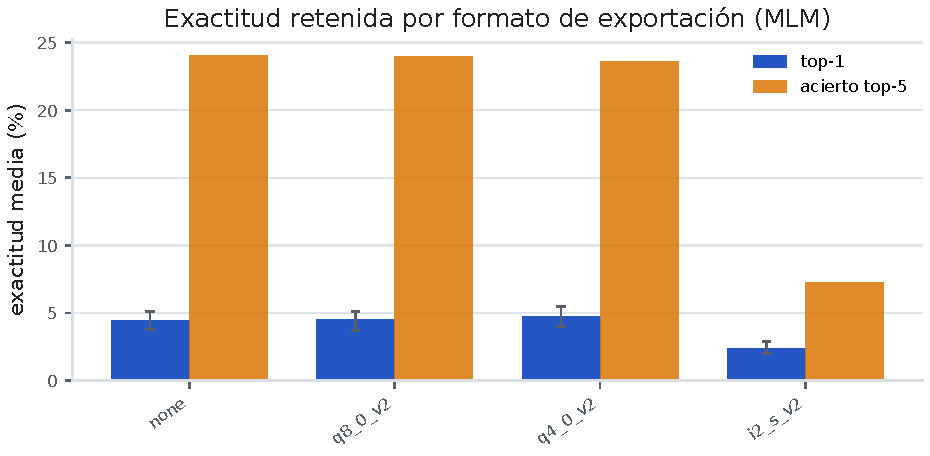
\includegraphics{../paper/figures/experiments/round3/inference_format_accuracy-es.pdf}}
\caption{Exactitud top-1 y top-5 retenida de la exportación sin cuantizar y de los tres códecs v2.}
\label{fig:r3-inference-format}
\end{figure}

La vista agregada (Figura~\ref{fig:r3-inference-format} y Tabla~\ref{tab:r3-formats}) dice que los pesos de 8 y 4 bits son esencialmente gratis a esta escala. Respecto de la exportación sin cuantizar, \texttt{q8\_0\_v2} cambia la exactitud top-1 en $+0,07$ puntos porcentuales y deja sin cambios el $99,2\%$ de los pares, con solo el $0,2\%$ degradado; \texttt{q4\_0\_v2} la cambia en $+0,33$ puntos con el $94,5\%$ sin cambios y el $1,7\%$ degradado. El códec de 2 bits es la excepción: \texttt{i2\_s\_v2} cambia la exactitud top-1 en $-2,03$ puntos de media, deja intacto el $73,2\%$ de los pares y degrada el $18,7\%$. Las filas \texttt{v1} se muestran en la tabla por completitud pero no son comparables con la base, porque sus máscaras son más difíciles: los mismos pares logran $14,4\%$ de top-5 con \texttt{v1} frente a $24,0\%$ con \texttt{hf\_none}.

\begin{table}[H]
\centering
\small
\caption{Exactitud retenida por formato de exportación (MLM): pares evaluados, top-1 y top-5 medios, delta medio frente a la exportación sin cuantizar, intervalo bootstrap del 95\% y fracción de pares que empeoran.}
\label{tab:r3-formats}
\begin{tabular}{lrrrcrr}
\toprule
Formato & $n$ & Top-1 & Top-5 & $\Delta$ (pp) & IC 95\% & Peor \\
\midrule
none & 653 & 4,46 & 24,0 & 0,000 & -- & 0,0\% \\
\texttt{q8\_0\_v1} & 653 & 2,87 & 14,4 & -1,663 & -2,406 / -0,788 & 22,2\% \\
\texttt{q8\_0\_v2} & 653 & 4,50 & 23,9 & +0,066 & -0,022 / +0,175 & 0,2\% \\
\texttt{q4\_0\_v1} & 653 & 2,72 & 14,1 & -1,816 & -2,560 / -0,919 & 22,2\% \\
\texttt{q4\_0\_v2} & 653 & 4,76 & 23,6 & +0,328 & +0,088 / +0,569 & 1,7\% \\
\texttt{i2\_s\_v1} & 653 & 0,83 & 3,2 & -3,719 & -4,375 / -3,040 & 24,2\% \\
\texttt{i2\_s\_v2} & 653 & 2,41 & 7,2 & -2,035 & -2,713 / -1,313 & 18,7\% \\
\bottomrule
\end{tabular}
\end{table}

La vista por muestra es más nítida que el agregado. Emparejando cada predicción cuantizada con la predicción base de la misma máscara, \texttt{q8\_0\_v2} coincide en el $99,5\%$ de las muestras (IC del 95\% del bootstrap por par), \texttt{q4\_0\_v2} en el $91,8\%$ y \texttt{i2\_s\_v2} en solo el $20,8\%$. El modelo de 2 bits no es una copia algo peor del profesor: es un modelo distinto que casualmente conserva el top-1 agregado en los pares cuya exactitud base ya era casi cero.

\begin{figure}[tbp]
\centering
\fitfigure{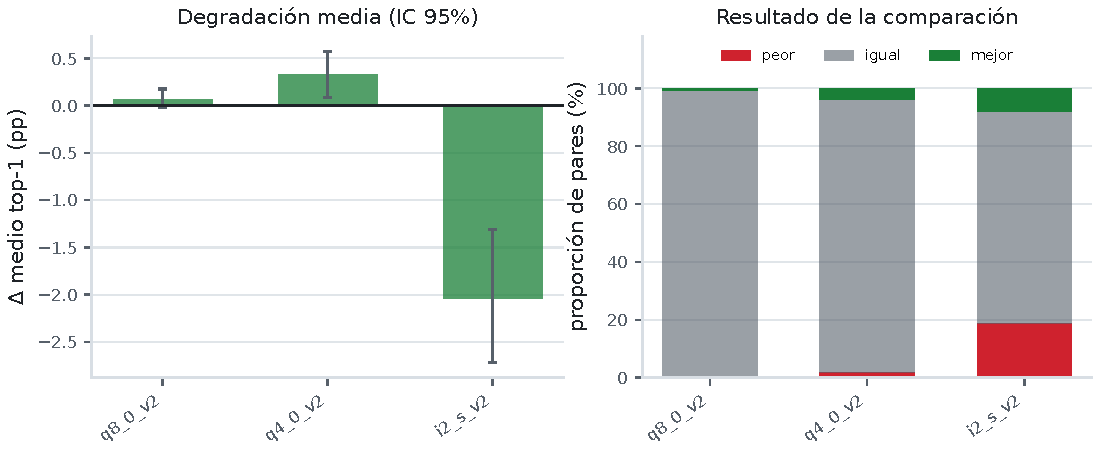
\includegraphics{../paper/figures/experiments/round3/quant_delta_dist-es.pdf}}
\caption{Delta medio de top-1 contra la exportación sin cuantizar (IC bootstrap del 95\%) y proporción de pares que empeoran, quedan igual o mejoran.}
\label{fig:r3-quant-delta}
\end{figure}
\begin{figure}[tbp]
\centering
\fitfigure{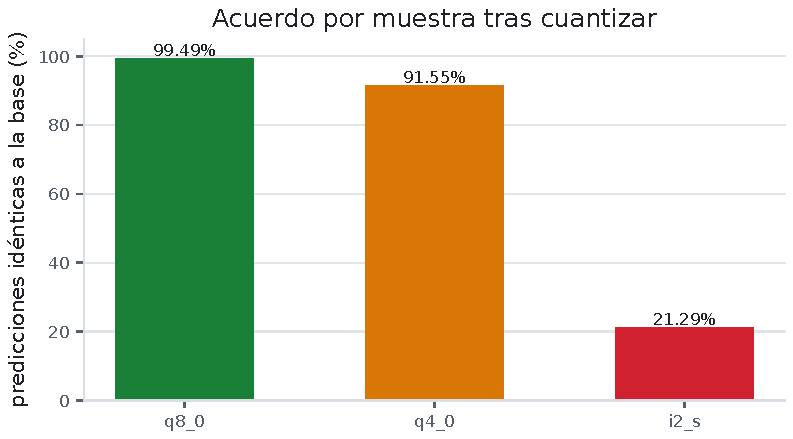
\includegraphics{../paper/figures/experiments/round3/quant_agreement-es.pdf}}
\caption{Acuerdo por muestra con las predicciones sin cuantizar para el runtime v2.}
\label{fig:r3-quant-agreement}
\end{figure}

Dos resultados negativos completan la sección. El número de parámetros no predice la robustez a la cuantización de 2 bits (Spearman $-0,11$ entre el delta de \texttt{i2\_s} y el recuento de parámetros), y la pérdida de entrenamiento no predice la calidad retenida (Spearman $+0,14$). A esta escala la única señal fiable es la comparación misma: medir la exportación cuantizada contra la no cuantizada, sobre las mismas muestras, y reportar el acuerdo en lugar del agregado.

\begin{figure}[tbp]
\centering
\fitfigure{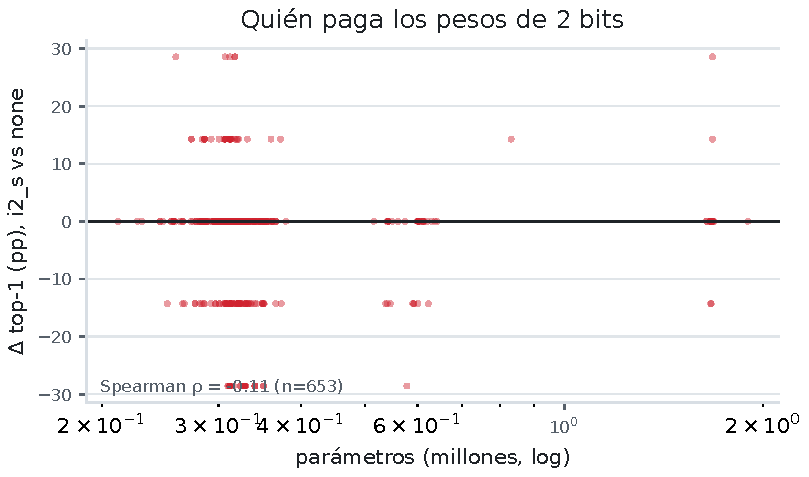
\includegraphics{../paper/figures/experiments/round3/quant_delta_vs_params-es.pdf}}
\caption{Delta de exactitud de 2 bits contra número de parámetros.}
\label{fig:r3-quant-params}
\end{figure}
\begin{figure}[tbp]
\centering
\fitfigure{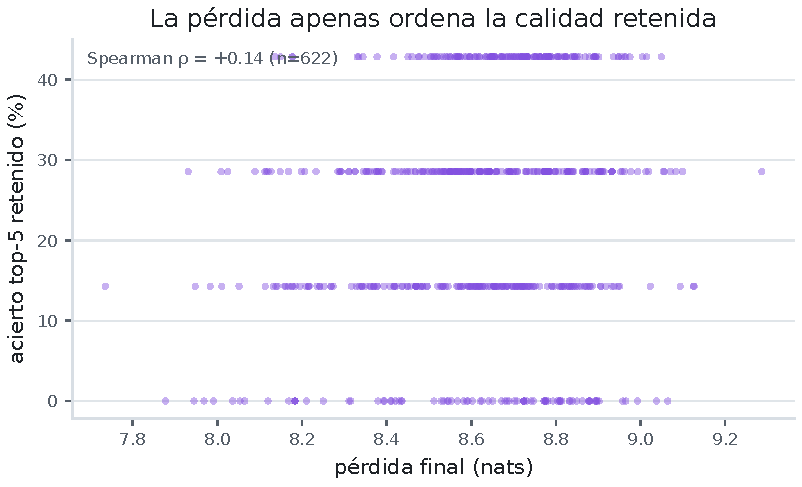
\includegraphics{../paper/figures/experiments/round3/train_vs_inference-es.pdf}}
\caption{Pérdida final de entrenamiento contra acierto top-5 retenido para los pares MLM.}
\label{fig:r3-train-inference}
\end{figure}

\subsection{Fiabilidad y taxonomía de fallos}
\label{sec:r3-reliability}

El entrenamiento es fiable: $1{,}643$ de $1{,}653$ corridas terminan bien (tasa de fallo $0,6\%$). Los diez fallos son pares híbridos que contienen \texttt{engram}; ocho salen con código 1 y dos con código 134 (SIGABRT), y ninguna otra familia falla. El fallo es estructural y no aleatorio---\texttt{engram} es el único mixer con un banco de memoria externo, y diez de los cincuenta y tres pares que lo usan fallan mientras los otros cuarenta y tres entrenan---y por eso el atlas sigue conteniendo todas las celdas: los diez pares fallidos están en la tabla de población pero ausentes de los análisis de pérdida e inferencia.

El resto del pipeline está más sano que en la ronda~2. La exportación a Transformers no falla nunca ($4{,}686$ registros, todos OK), la evaluación de inferencia falla una vez (una corrida \texttt{pape\_efficient}) y el único problema sistémico es la etapa de despliegue excluida arriba. El registro de etapas (Figura~\ref{fig:r3-stage-status}) hace visible la asimetría: entrenamiento y exportación están casi enteramente en verde, la inferencia está en verde con una fila roja y el despliegue es la única etapa con un bloque rojo grande.

\begin{figure}[tbp]
\centering
\fitfigure{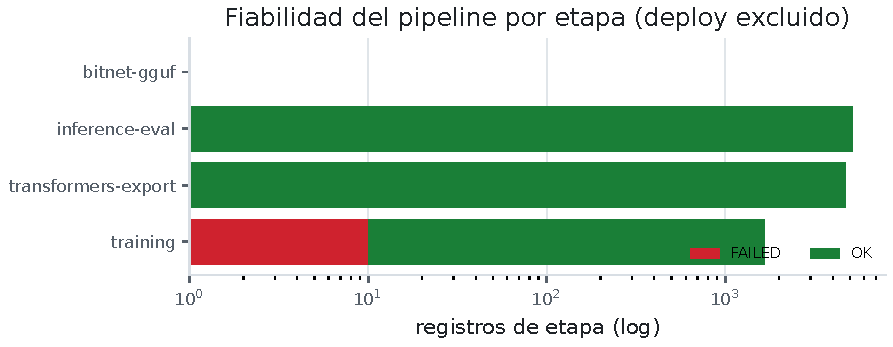
\includegraphics{../paper/figures/experiments/round3/stage_status-es.pdf}}
\caption{Estado del pipeline por etapa, sin despliegue.}
\label{fig:r3-stage-status}
\end{figure}

\subsection{Correlaciones}

La Figura~\ref{fig:r3-correlation} es la matriz de Spearman de las variables medidas sobre los $1{,}431$ pares. Las correlaciones fuertes no triviales son las que describen el calendario y no la arquitectura: el tiempo de entrenamiento crece con el número de épocas ($+0,74$), el rendimiento es casi el inverso del tiempo por paso ($-0,95$) y la pérdida media baja a medida que el calendario se alarga ($-0,76$). El número de parámetros se correlaciona moderadamente con la pérdida ($-0,42$) y con la magnitud del gradiente ($+0,47$) y débilmente con el tiempo de pared ($+0,23$), la forma cuantitativa de la ley de coste débil de la sección anterior.

\begin{figure}[tbp]
\centering
\fitfigure{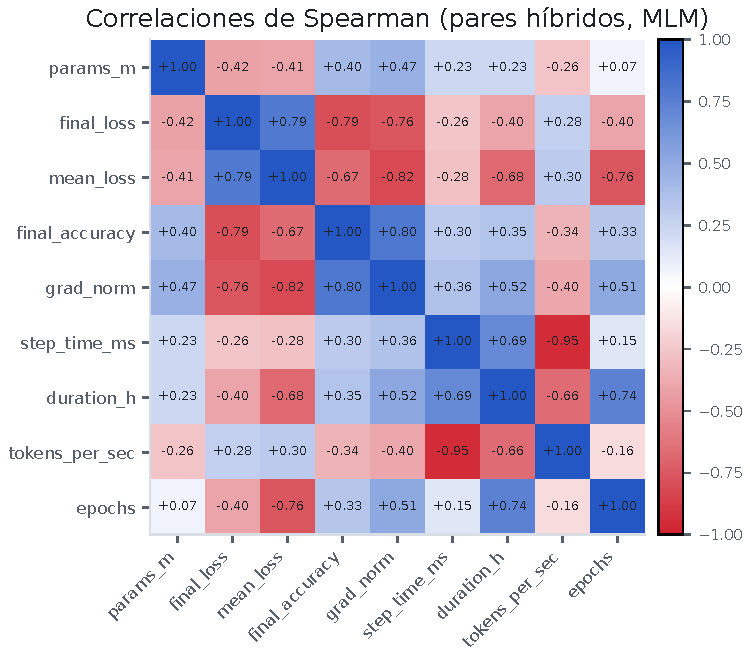
\includegraphics{../paper/figures/experiments/round3/correlation-es.pdf}}
\caption{Correlaciones de Spearman de las variables medidas sobre los pares híbridos.}
\label{fig:r3-correlation}
\end{figure}

\subsection{Resumen de hallazgos}

\begin{enumerate}[leftmargin=1.4em,itemsep=2pt]
\item El atlas completo es medible en una semana de un solo host de CPU: $1{,}653$ corridas, $20,5$ millones de pasos, $3{,}668$ horas, una tasa de fallo de entrenamiento del $0,6\%$ y ningún paso con NaN.
\item La pila de mixers domina el espacio de diseño. El mejor par alcanza $7,736$ nats y el peor $9,70$, mientras que las ablaciones de optimizador, normalización y codificación posicional mueven la pérdida menos que la dispersión entre pares.
\item El tamaño ayuda pero no decide: la correlación de rango entre parámetros y pérdida es $-0,42$, y los mixers más baratos se reparten a ambos lados de la mediana.
\item El aprendizaje es rápido y el ranking se decide temprano: el par mediano alcanza el 90\% de su caída de pérdida al $41\%$ del calendario y los diez mejores se separan de la población en el primer 15\%.
\item La presión del gradiente es estable y específica por bloque: dominan la cabeza ($3,66$), la atención ($2,12$) y la FFN ($0,71$), los coeficientes de variación de los bloques activos se quedan por debajo de 0,35 y el orden de los bloques es constante en la campaña.
\item El recorte es rutina, no excepción: la mediana del cociente de recorte es $1,04$ y el $51,6\%$ de las corridas recortan de media, lo que cambia la lectura de las normas de gradiente a cantidades posteriores al recorte.
\item El tiempo de entrenamiento es casi independiente del número de parámetros con un calendario fijo (exponente log-log $0,25$, $R^2=0,06$): lo domina el número de pasos, y los pares híbridos absorben el $90,0\%$ de las $3{,}668$ horas.
\item La cuantización a 8 y 4 bits es esencialmente sin pérdida en el runtime \texttt{v2} ($99,5\%$ y $91,8\%$ de acuerdo por muestra), mientras que los pesos de 2 bits cambian el modelo cualitativamente ($20,8\%$ de acuerdo, $-2,03$ puntos de top-1).
\item El pipeline es fiable salvo la etapa de despliegue, cuyo error de payload de configuración está documentado y excluido; las rutas de exportación y evaluación están limpias.
\item La ronda hereda la advertencia central de la ronda~2: la pérdida de entrenamiento y la calidad retenida son casi incorrelacionadas ($+0,14$), así que el atlas debe leerse como un mapa de velocidad y estabilidad de aprendizaje, no como una tabla de líderes.
\end{enumerate}

\subsection{Reproducir este apéndice}

El apéndice lo generan cuatro scripts en \texttt{experimentos/3/report/}, en orden:

\begin{verbatim}
python experimentos/to_csv.py 3                       # exportación plana a CSV
python experimentos/3/report/build_data.py            # master/epochs/inference
python experimentos/3/report/make_paper_figures.py    # PDF/SVG, ambos idiomas
python experimentos/3/report/make_report.py           # estadísticas + este apéndice
\end{verbatim}

\texttt{build\_data.py} recorre una sola vez el log por paso de 6,6\,GB (unos diez minutos) y cachea todos los agregados; los otros tres scripts tardan segundos. \texttt{make\_report.py} escribe \texttt{out/stats.json} con todos los números citados arriba, así que cualquier afirmación se puede rastrear hasta el CSV que la produjo.
